% Статья о GORKY. Сборка: tectonic gorky.tex (из папки docs/paper) → gorky.pdf.
\documentclass[10pt,a4paper,twocolumn]{article}

\usepackage[a4paper,top=2.2cm,bottom=2.4cm,left=2cm,right=2cm,columnsep=0.7cm]{geometry}
\usepackage{fontspec}
\usepackage[russian]{babel}
\setmainfont{LibertinusSerif}[Extension=.otf,UprightFont=*-Regular,BoldFont=*-Bold,
  ItalicFont=*-Italic,BoldItalicFont=*-BoldItalic]
\setsansfont{LibertinusSans}[Extension=.otf,UprightFont=*-Regular,BoldFont=*-Bold,
  ItalicFont=*-Italic]
\setmonofont{DejaVuSansMono}[Extension=.ttf,Scale=0.82,BoldFont=*-Bold]

\usepackage{graphicx}
\usepackage{booktabs}
\usepackage{tabularx}
\usepackage{array}
\usepackage{enumitem}
\usepackage{caption}
\usepackage[round]{natbib}
\usepackage{xcolor}
\usepackage[colorlinks=true,linkcolor=blue!50!black,citecolor=blue!50!black,
  urlcolor=blue!50!black]{hyperref}
\usepackage{tikz}
\usetikzlibrary{positioning,arrows.meta,fit,calc}

\setlist{nosep,leftmargin=1.2em}
\captionsetup{font=small,labelsep=colon}
\setlength{\parskip}{0pt}
\renewcommand{\bibname}{Литература}
\renewcommand{\refname}{Литература}
\newcommand{\code}[1]{\texttt{#1}}
\newcolumntype{L}{>{\raggedright\arraybackslash}X}

\tikzset{
  box/.style={draw=black!70,rounded corners=2pt,fill=blue!4,align=center,
    font=\small,inner sep=4pt,minimum height=0.95cm},
  core/.style={box,fill=orange!10},
  store/.style={box,fill=green!7},
  arr/.style={-{Stealth[length=2mm]},black!70},
  lbl/.style={font=\scriptsize,text=black!70,align=center},
}

\title{\bfseries GORKY: голосовой ассистент задач и встреч,\\
  в котором модель выбирает действие, а исполняет код}
\author{%
  \textbf{Родион Музыкант, Анастасия Безусова, Илья Бурмистров,}\\
  \textbf{Мария Ворона, Денис Чичеров, Давид Егиазарян}\\[2pt]
  НИУ ВШЭ — Нижний Новгород\\[2pt]
  \small\url{https://github.com/anastbezu/gorkycode-test}\quad·\quad\url{https://gorky.bond}}
\date{}

\begin{document}
\maketitle

\begin{abstract}
GORKY — голосовой ассистент, который ведёт личные задачи, напоминания и встречи по
свободной речи: создаёт записи, показывает планы за период, находит старые записи по
смыслу, переносит и отменяет их, переспрашивает, когда данных не хватает. Ключевое
решение — разделение ролей: языковая модель за один вызов на реплику выбирает одно из
восьми действий и заполняет его аргументы по строгой схеме, а проверки, поиск цели,
запись в базу и текст ответа выполняет код. Поиск устроен в два уровня: «точно» по
основам слов и «похоже» по векторам; менять запись можно только по точному совпадению.
Качество агента измеряет бенчмарк из 581 кейса (747 реплик) в девяти наборах на
настоящей модели и настоящей базе: пройдено 95,9\,\% кейсов, выбор действия —
macro-F1 0,967, медиана времени реплики — 1,12\,с. Поиск на 457 запросах с ответом
находит нужную запись в 96,5\,\% случаев и ни разу не выбрал чужую запись для изменения
среди 587 целей.
\end{abstract}

\section{Введение}

Фраза «перенеси её на пятницу» короткая, но для ассистента в ней несколько задач:
понять, что это перенос, а не новая запись; найти, какую запись пользователь называет
«её»; вычислить дату ближайшей пятницы от текущего момента в его часовом поясе;
сохранить прежнее время; проверить, что новая дата не в прошлом, и предупредить о
пересечении с другой встречей. Если всё это поручить языковой модели целиком, ошибки
трудно заметить: модель может ответить «Готово», не сохранив запись, изменить похожую,
но чужую запись или ошибиться в дате на неделю.

GORKY решает это разделением ответственности:
\begin{itemize}
  \item \textbf{один вызов модели на реплику}: модель возвращает одно действие из восьми
    по строгой схеме (tool calling), всё остальное делает код; нет многошаговых
    рассуждений и повторных вызовов — поведение предсказуемо, запросов к модели мало;
  \item \textbf{состояние разговора на сервере}: вместо истории сообщений модель получает
    короткую выжимку — показанные записи под номерами, запись «в фокусе», черновик;
  \item \textbf{безопасная цель изменения}: код меняет только точно найденную запись,
    похожую лишь предлагает вопросом, любое изменение откатывается словом «верни»;
  \item \textbf{двухуровневый поиск}: «точно» по основам слов и «похоже» по векторам
    локальной модели эмбеддингов;
  \item \textbf{бенчмарк}: 581 кейс в девяти наборах, прогон на настоящей модели и базе,
    метрики по действию, по каждому полю и по времени ответа.
\end{itemize}

\section{Архитектура}

\begin{figure*}[t]
\centering
\resizebox{\textwidth}{!}{%
\begin{tikzpicture}[node distance=0.55cm and 0.75cm]
  \node[box] (ui) {Браузер\\{\scriptsize чат, микрофон, «Мои дела»,}\\{\scriptsize календарь, озвучка ответа}};
  \node[box,right=1.1cm of ui] (api) {API FastAPI\\{\scriptsize \code{/api/chat}, \code{/api/items},}\\{\scriptsize \code{/api/stt}}};
  \node[box,above=0.5cm of api] (stt) {Распознавание речи\\{\scriptsize Gemini, до 30\,с}};
  \node[core,right=1.1cm of api] (agent) {Агент\\{\scriptsize состояние разговора,}\\{\scriptsize исполнение, ответ по шаблону}};
  \node[box,above=0.5cm of agent] (llm) {LLM\\{\scriptsize один вызов, 8 инструментов}};
  \node[box,right=1.1cm of agent,yshift=0.75cm] (svc) {Сервисы\\{\scriptsize проверки, пересечения,}\\{\scriptsize дубли, откат}};
  \node[box,right=1.1cm of agent,yshift=-0.75cm] (search) {Поиск\\{\scriptsize «точно» по словам,}\\{\scriptsize «похоже» по векторам}};
  \node[store,right=0.9cm of svc,yshift=-0.75cm] (db) {PostgreSQL\\+ pgvector\\{\scriptsize записи, состояние,}\\{\scriptsize векторы, учётки}};
  \node[box,below=0.5cm of api] (gcal) {Google Календарь\\{\scriptsize после коммита}};

  \draw[arr] (ui.north) |- node[lbl,pos=0.75,above]{аудио} (stt.west);
  \draw[arr] (stt.south) -- node[lbl,right]{текст} (api.north);
  \draw[arr] ([yshift=2pt]ui.east) -- node[lbl,above]{текст} ([yshift=2pt]api.west);
  \draw[arr] ([yshift=-2pt]api.west) -- node[lbl,below]{ответ} ([yshift=-2pt]ui.east);
  \draw[arr] (api) -- (agent);
  \draw[arr] ([xshift=-3pt]agent.north) -- node[lbl,left]{выжимка\\и фраза} ([xshift=-3pt]llm.south);
  \draw[arr] ([xshift=3pt]llm.south) -- node[lbl,right]{действие\\и поля} ([xshift=3pt]agent.north);
  \draw[arr] (agent.east) -- ++(0.45,0) |- (svc.west);
  \draw[arr] (agent.east) -- ++(0.45,0) |- (search.west);
  \draw[arr] (svc.east) -- ++(0.25,0) |- ([yshift=4pt]db.west);
  \draw[arr] (search.east) -- ++(0.25,0) |- ([yshift=-4pt]db.west);
  \draw[arr] (api.south) -- (gcal.north);
\end{tikzpicture}}
\caption{Архитектура GORKY. Голос превращается в текст на сервере, дальше путь общий для
голоса и клавиатуры. Агент вызывает модель один раз на реплику; запись в базу, поиск и
текст ответа — код. Запись и состояние разговора сохраняются одним коммитом.}
\label{fig:arch}
\end{figure*}

Система — веб-приложение из трёх контейнеров: PostgreSQL с расширением pgvector,
бэкенд на Python 3.13 и FastAPI, страница на React и TypeScript (рис.~\ref{fig:arch}).
Голос распознаётся на сервере моделью Gemini (запись до 30\,с), после чего путь
запроса не зависит от того, говорил пользователь или печатал. Ответ озвучивается
голосом браузера: один текст служит и для экрана, и для речи.

Бэкенд разделён на модули с договорёнными контрактами: \code{api} — HTTP; \code{agent} —
разговор и вызов модели; \code{services} — правила записей, которыми пользуются и агент,
и кнопки интерфейса без модели; \code{search} — поиск; \code{db} — модели SQLAlchemy и
миграции Alembic. Модель доступна через OpenAI-совместимый API, поэтому провайдер
меняется настройкой. Запись и состояние разговора сохраняются в одной транзакции:
ассистент не может «запомнить» изменение, которого нет в базе, и наоборот. Поддержаны
гости без регистрации и учётки по логину и паролю; записи учётки можно отправлять в
отдельный Google Календарь.

\section{Агент}

\subsection{Один вызов модели на реплику}

Модель получает системный промпт с текущим временем, днём недели и календарём на две
недели, выжимку состояния разговора и фразу пользователя, и обязана вызвать ровно один
инструмент (табл.~\ref{tab:tools}). Аргументы описаны моделями Pydantic, из которых
генерируется JSON-схема инструментов; ответ модели проверяется той же схемой. Дальше
работает код: исполняет действие, обновляет состояние и собирает ответ по шаблону.
Текст «Готово, встреча создана» никогда не пишет модель — только код после успешной
записи.

\begin{table}[t]
\centering\small
\begin{tabularx}{\columnwidth}{@{}lL@{}}
\toprule
Инструмент & Когда \\
\midrule
\code{create\_record} & создать задачу, напоминание, встречу \\
\code{list\_records} & записи за период: «что у меня завтра» \\
\code{search\_records} & по теме или человеку: «встреча с Иваном» \\
\code{update\_record} & перенести, переименовать, сдвинуть \\
\code{set\_status} & выполнено, отменено, вернуть в активные \\
\code{undo\_last} & «верни как было» \\
\code{ask\_user} & не хватает данных — вопрос \\
\code{help} & справка или посторонняя тема \\
\bottomrule
\end{tabularx}
\caption{Восемь инструментов агента.}
\label{tab:tools}
\end{table}

Часть реплик не требует модели вовсе. Отказ посреди уточнения («не надо»,
«передумал») код распознаёт по списку фраз и сбрасывает черновик; ответ «номер 3» на
вопрос «какую?» код разбирает сам.

\subsection{Состояние разговора}

Вместо истории сообщений на сервере хранится структура: \code{shown} — записи в том
порядке, в каком их назвали пользователю; \code{focus} — запись, о которой речь
(«её», «эту»); \code{pending} и \code{missing} — черновик создания и чего в нём не
хватает; \code{candidates} — записи для выбора; \code{last\_action} — прежние значения
последнего изменения для отката. В промпт попадает короткая текстовая выжимка этой
структуры. Так «вторую» превращается в номер из \code{shown}, «нет, в 16» — в правку
записи в фокусе, а ответ «в 15» на вопрос о времени — в дополнение черновика.

\subsection{Цель изменения}

Для переноса и смены статуса модель не передаёт идентификаторов: она описывает цель —
номером на экране, словом «её», текстом с названным временем или фильтром для «отмени
всё на завтра». Переводит описание в запись код (функция \code{find\_target}):
\begin{itemize}
  \item одна точная запись — действие исполняется;
  \item несколько — код ничего не меняет и спрашивает «какую?» со списком;
  \item точных нет, есть похожие — вопрос «Точно такой нет. Может, эту?»;
  \item массовое действие — подтверждение «Отменить 5 созвонов?», не больше 20 записей.
\end{itemize}
Похожая запись без ответа пользователя не меняется никогда. Отмена сразу исполняется,
но удаление мягкое: «верни» восстанавливает прежнее состояние, «нет, не эту, а ту»
откатывает действие и применяет его к другой записи.

\subsection{Даты и время}

Модель возвращает даты в ISO 8601 со смещением пояса пользователя, а промпт задаёт
умолчания: «в 3» без «утра» — 15:00 (часы 1–7 считаются дневными), «утром» — 09:00,
«вечером» — 18:00; день недели, совпадающий с сегодняшним, — через неделю; время без
дня — сегодня; «до конца недели» — срок в воскресенье 23:59. Встреча без времени
сохраняется только после вопроса «На какое время?». Код проверяет, что дата не в
прошлом и конец позже начала, не создаёт точный дубль и сообщает о пересечении встреч,
не блокируя сохранение.

\section{Поиск}

Поиск отвечает на «когда у меня была встреча с Иваном» и находит цель изменения.
Он устроен в два уровня.

\textbf{«Точно».} Название записи и запрос разбираются на слова; каждое слово
сравнивается по основе (стеммер Snowball, \citealp{porter2001snowball}), по лемме
(pymorphy, \citealp{korobov2015morphological}) и нечётко — с порогом сходства 85 для
опечаток. Служебные слова («с», «про», «по») не учитываются; слово типа («встречу»,
«задачу») совпадает, если оно есть в названии или запись этого типа: «встречу с Севером»
находит «Созвон с Севером». Запись подходит, если совпали все значимые слова запроса.

\textbf{«Похоже».} Если точных нет, запрос и названия сравниваются по векторам модели
\code{rubert-mini-frida} \citep{frida2024} размерности 312 в pgvector; показываются до
10 записей со сходством не ниже 0,45. Модель работает на сервере — без ключа, сети и
лимитов. Результаты упорядочены по близости ко времени: сначала ближайшие будущие,
затем прошедшие от новых к старым.

\textbf{Замер.} На стартовом наборе из 1000 записей поиск проверен двумя наборами
(табл.~\ref{tab:search}). Базовый — 30 запросов с ответом и 6 без ответа; расширенный —
619 запросов по группам граничных случаев (падежи, опечатки, сокращения, фильтры) и 587
целей изменения. Главное свойство для безопасности — ни одна из 587 целей не привела к
действию над чужой записью. Слабое место — сокращения и сленг («ТЗ», «КП», «презентуха»):
их не ловит ни сравнение слов, ни небольшая модель эмбеддингов.

\begin{table}[t]
\centering\small
\begin{tabularx}{\columnwidth}{@{}Lr@{}}
\toprule
Метрика & Значение \\
\midrule
Базовый набор: hit@5 & 29/30 \\
Расширенный: нашёл подходящую & 441/457 (96,5\,\%) \\
\quad падежи имён и компаний & 69/69 \\
\quad человек + тема, компания + тема & 147/147 \\
\quad опечатки & 28/37 \\
\quad синонимы и сокращения & 16/21 \\
«Точно» на запросах без ответа & 0 \\
Цели изменения: чужая запись & 0 из 587 \\
\bottomrule
\end{tabularx}
\caption{Поиск на стартовом наборе из 1000 записей.}
\label{tab:search}
\end{table}

\section{Оценка агента}

\subsection{Наборы и протокол}

Кейс — фраза пользователя или диалог из 2–4 реплик с ожиданием на каждой реплике:
какой инструмент вызван, значения его полей (тип, название, начало, срок, период,
запрос, цель изменения) и исход (исполнено, ждёт ответа, ждёт выбора). Проверяются
только заданные в ожидании поля; названия и запросы — по основам слов, даты — до
минуты в поясе пользователя. «Сейчас» во всех кейсах — среда 21.10.2026, 10:00,
Europe/Moscow.

Набор \code{test-cases} составлен командой и включает все примеры из задания. Восемь
наборов по действиям сгенерированы моделью Gemini 3.8 Flash (high reasoning) по
контрактам модулей: ожидание — только то, что однозначно следует из контракта, без
чтения кода агента. Агент в замере работает на другой модели —
\code{gemini-3.5-flash-lite}, поэтому модель не проверяет сама себя.

Прогон идёт через ту же функцию обработки реплики, что и API, с настоящей моделью и
PostgreSQL с настоящим поиском; каждый кейс исполняется в своей транзакции с откатом.

\subsection{Метрики}

Кейс пройден, если верны все его реплики. Выбор инструмента оценивается по матрице
ошибок: precision, recall и F1 по каждому инструменту и macro-F1 — среднее F1. Для
полей считается доля верных значений; если инструмент выбран неверно, все поля реплики
засчитываются неверными. Время
реплики — от текста пользователя до готового ответа, включая исполнение на базе.

\subsection{Результаты}

\begin{table}[t]
\centering\small
\begin{tabularx}{\columnwidth}{@{}lLrr@{}}
\toprule
Набор & Что проверяет & Кейсов & Пройдено \\
\midrule
test-cases & задание и сценарии & 176 & 98,3\,\% \\
create & создание & 75 & 98,7\,\% \\
list & список за период & 50 & 96,0\,\% \\
search & поиск & 50 & 100\,\% \\
update & изменение & 60 & 95,0\,\% \\
status & статус, массовые & 50 & 88,0\,\% \\
dialog & уточнение, выбор & 50 & 92,0\,\% \\
traps & подвохи выбора & 50 & 92,0\,\% \\
undo & откат & 20 & 95,0\,\% \\
\midrule
Всего & & 581 & 95,9\,\% \\
\bottomrule
\end{tabularx}
\caption{Доля пройденных кейсов по наборам; 747 реплик.}
\label{tab:datasets}
\end{table}

Агент прошёл 557 из 581 кейса (95,9\,\%, табл.~\ref{tab:datasets}). Выбор
инструмента — macro-F1 0,967 (рис.~\ref{fig:tools}): точнее всего создание (F1 0,998)
и список (0,996), слабее всего вопрос \code{ask\_user} (recall 0,77) — иногда агент
действует там, где следовало переспросить. Название записи верно в 199 из 199 реплик,
тип — в 218 из 218, начало с признаком «время названо» — в 97,3\,\%. Медиана времени реплики — 1,12\,с,
95-й процентиль — 1,81\,с.

\begin{figure}[t]
\centering
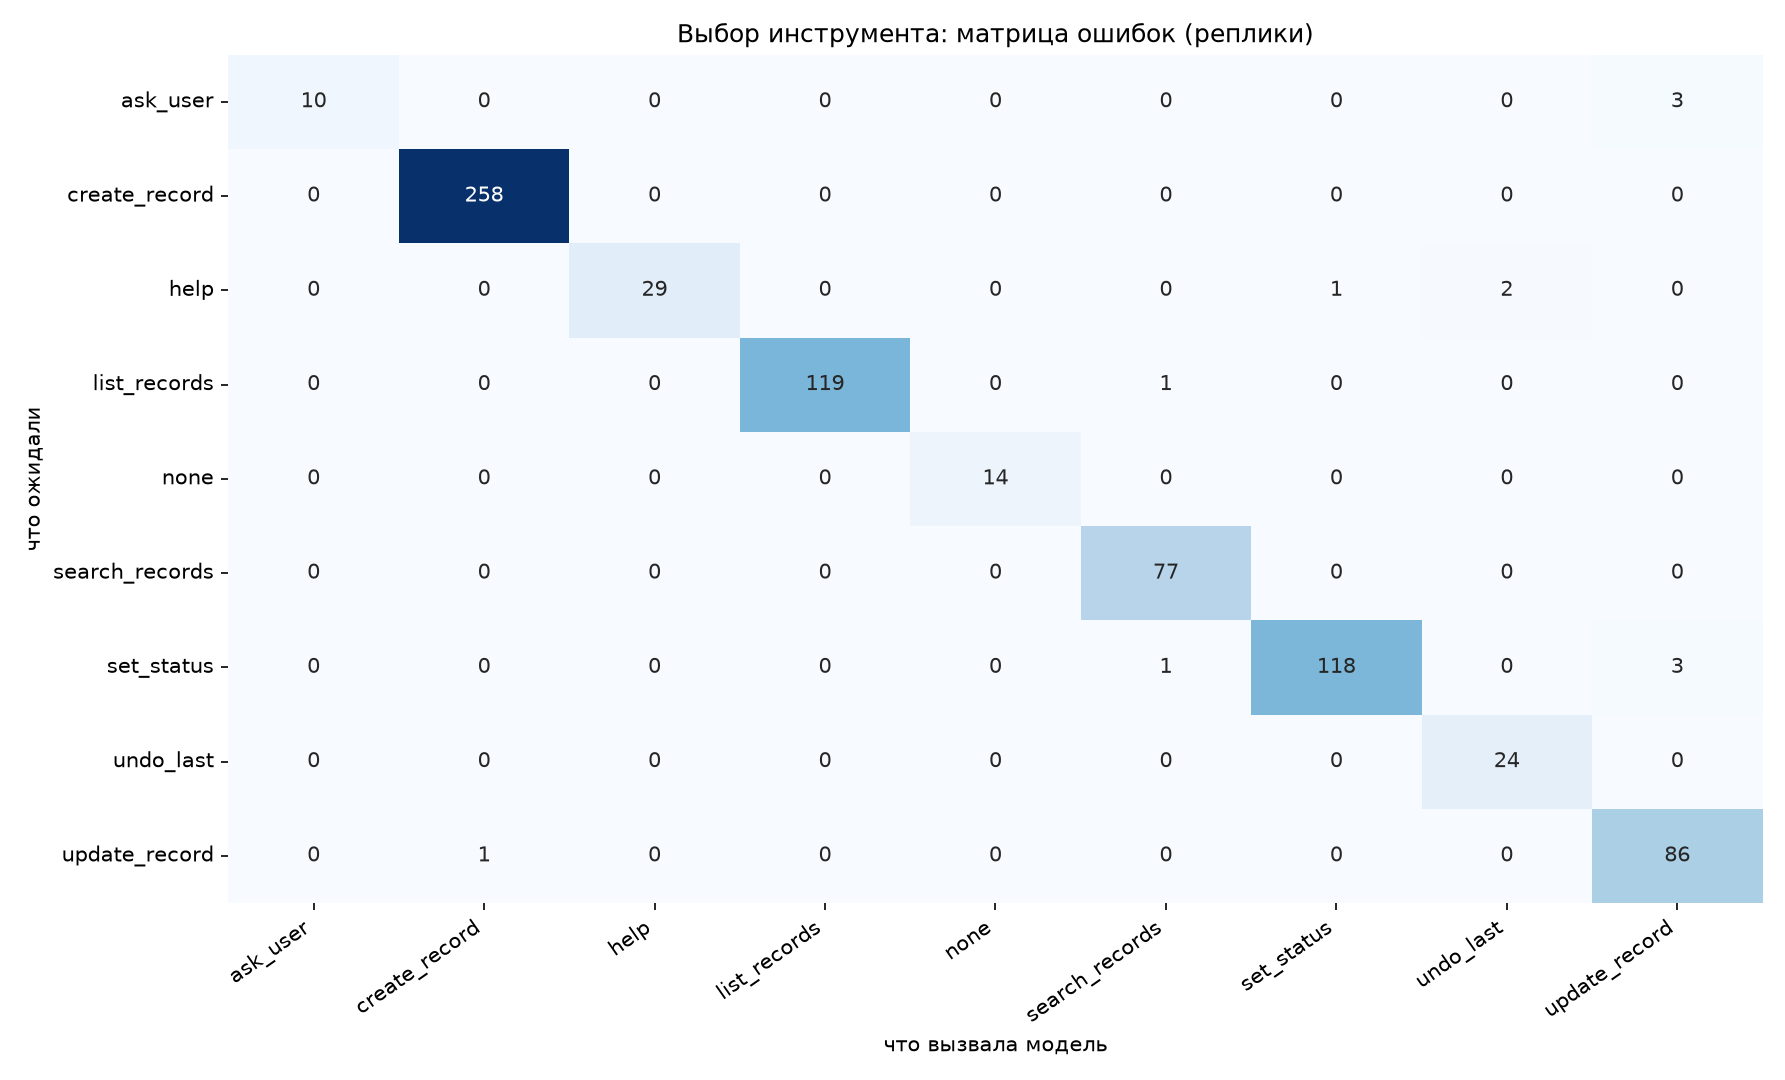
\includegraphics[width=\columnwidth]{../../backend/eval/reports/agent-final/tools.png}
\caption{Матрица ошибок выбора инструмента по 747 репликам: строки — что ожидали,
столбцы — что вызвала модель. \code{none} — ответ кода без модели (отказ).}
\label{fig:tools}
\end{figure}

\subsection{Разбор ошибок}

Все 24 непройденных кейса разобраны вручную:
\begin{itemize}
  \item \textbf{не тот инструмент — 9}: изменение вместо смены статуса в «нет, не с
    Ярославом, а с Ростиславом», поиск вместо отметки «готово, смету отправил»,
    правка вместо вопроса, когда ответ «в 16» пришёл после смены темы;
  \item \textbf{даты и время — 7}: «в среду», сказанное в среду, — сегодня вместо
    следующей недели; «в восемь» — 20:00 вместо 08:00; начало у задачи, где назван
    только срок;
  \item \textbf{отрицание — 3}: «не отменяй встречу с Иваном» агент исполняет как
    откат;
  \item \textbf{две команды в фразе — 2}, \textbf{цель и статус — 2};
  \item \textbf{поиск — 1}: «закрой задачу про печать» не находит «Распечатать
    договор»: однокоренные слова с приставкой не совпадают по основе.
\end{itemize}
Двадцать три ошибки из двадцати четырёх — ошибки понимания модели; их направление
понятно: отрицание и даты закрываются вычислением дат в коде (модель отдаёт
сказанное, «пятница, 15:00», а дату считает функция) и отдельным действием «отказ».

\section{Ограничения}

\begin{itemize}
  \item Один прогон на одной модели: разброс ответов между прогонами (pass$^k$,
    \citealp{yao2024taubench}) и другие модели не измерены.
  \item Восемь из девяти наборов сгенерированы моделью по контрактам: в спорных
    формулировках эталон следует контракту и может расходиться с ожиданием живого
    пользователя.
  \item Проверяются вызов, поля и исход действия, а не формулировка ответа; голосовой
    тракт (распознавание и озвучка) в замер не входит.
  \item Агент исполняет только первую команду из фразы, кроме нескольких созданий;
    повторяющихся записей нет.
  \item Поиск не знает сокращений и сленга без словаря синонимов.
\end{itemize}

\section{Заключение}

Разделение «модель выбирает действие, код исполняет» делает поведение голосового
ассистента проверяемым: каждое действие — типизированный вызов, который можно сравнить
с эталоном поле за полем. На 581 кейсе агент выбирает верное действие с macro-F1 0,967
и проходит 95,9\,\% сценариев, а поиск ни разу не выбрал чужую запись для изменения.
Наборы, ответы агента на каждый кейс и отчёты лежат в репозитории
(\code{backend/eval/}) и пересобираются одной командой.

\bibliographystyle{plainnat}
\begin{thebibliography}{9}
\expandafter\ifx\csname url\endcsname\relax\def\url#1{\texttt{#1}}\fi

\bibitem[Korobov(2015)]{korobov2015morphological}
Mikhail Korobov. 2015. Morphological analyzer and generator for Russian and Ukrainian
languages. In \emph{Analysis of Images, Social Networks and Texts (AIST 2015)},
pages 320--332.

\bibitem[Porter(2001)]{porter2001snowball}
Martin F. Porter. 2001. Snowball: A language for stemming algorithms.
\url{https://snowballstem.org}.

\bibitem[rubert-mini-frida()]{frida2024}
rubert-mini-frida: компактная модель эмбеддингов для русского языка, дистилляция модели
FRIDA. \url{https://huggingface.co/sergeyzh/rubert-mini-frida}.

\bibitem[Yao et~al.(2024)]{yao2024taubench}
Shunyu Yao, Noah Shinn, Pedram Razavi, and Karthik Narasimhan. 2024. $\tau$-bench: A
benchmark for tool-agent-user interaction in real-world domains.
\emph{arXiv preprint arXiv:2406.12045}.

\end{thebibliography}

\end{document}
